
\documentclass{article}
\usepackage{v-problem}
\vgeometry
\usepgflibrary{easing}

\begin{document}
\vtitle[ELECTROSTATICS]

\def\pn{05}
\def\book{Irodov}
\def\page{106}
\def\gdrive{https://drive.google.com/drive/folders/1hHnYe1D6MhqnXqv0GsfC8Xyu778mHm-8?usp=share_link}

\def\question{
Two positive charges $q_1$ and $q_2$ are located at the points with radius vectors $\vec{r}_1$ and $\vec{r}_2$. Find a negative charge $q_3$ and a radius vector $\vec{r}_3$ of the point at which it has to be placed for the force acting on each of the three charges to be equal to zero.
}

\vspace*{\fill}
\begin{tikzpicture}
	\node[qnumber] (n) at (0, 0)[scale=2] {$\pn.$};
	\node[question] (q) [right=2mm of n.east] {\question};
	\tzline[divider]<-0.125, 0> (q.north west)(q.south west);
	\node[format] (f) at  (q.south east){[\book \quad \page]};
\end{tikzpicture}	
\vspace*{\fill}

\begin{center}
\begin{tikzpicture}
\tzcoor*(0, 0)(O){$O$}[bl]
\tzcoor*(70:3)(Q1){$q_1$}[br](5pt)
\tzcoor*(15:5)(Q2){$q_2$}[br](5pt)
\tzcoor*(35:4.5)(Q3){$q_3$}[b](5pt)
\tzaxes(-0.5, -0.5)(8,4){$x$}{$y$}
	\tzline[->](O)(Q1){$\vec{r}_1$}[mr]
	\tzline[->](O)(Q2){$\vec{r}_2$}[mb]
	\tzline[->](O)(Q3){$\vec{r}_3$}[mb]
\end{tikzpicture}
\end{center}
\vspace*{\fill}
\pagebreak

\vtitle[\texttt{Solution}]

\begin{center}
\begin{tikzpicture}
\def\v@f{60}
\def\fps{60}
\def\t{sinestep(0, \fps, \v@f)}
\tzcoor*(0, 0)(O){$O$}[bl]
\tzcoor*(70:3)(Q1){$q_1$}[br](5pt)
\tzcoor*(15:5)(Q2){$q_2$}[br](5pt)
\tzcoor*(35:{\t*4.5})(Q3){$q_3$}[b](5pt)
\tzaxes(-0.5, -0.5)(8,4){$x$}{$y$}
	\tzline[->](O)(Q1){$\vec{r}_1$}[mr]
	\tzline[->](O)(Q2){$\vec{r}_2$}[mb]
	\tzline[->](O)(Q3){$\vec{r}_3$}[mb]
	\tzline[->](Q3)($(Q3)!0.3!(Q1)$){$\vec{F}_{31}$}[l]
	\tzline[->](Q3)($(Q3)!0.3!(Q2)$){$\vec{F}_{32}$}[r]
	\tzline[->](Q2)($(Q2)!0.3!(Q3)$){$\vec{F}_{23}$}[l]
	\tzline[->](Q2)($(Q2)!-0.2!(Q1)$){$\vec{F}_{21}$}[r]
	\tzline[->](Q1)($(Q1)!0.3!(Q3)$){$\vec{F}_{13}$}[r]
	\tzline[->](Q1)($(Q1)!-0.2!(Q2)$){$\vec{F}_{12}$}[l]
\end{tikzpicture}
\end{center}

\addtolength{\jot}{3ex}
\begin{align}
\intertext{Net force on $q_1$ must be zero}
\vec{F}_{12} + \vec{F}_{13} &= 0\\
\intertext{Net force on $q_2$ must be zero}
\vec{F}_{21} + \vec{F}_{23} &= 0\\
\intertext{Net force on $q_3$ must be zero}
\vec{F}_{31} + \vec{F}_{32} &= 0
\end{align}
\pagebreak

\def\RPOTH{\left(\vec{r}_1-\vec{r}_3\right)}
\def\RMOTH{\left|\vec{r}_1-\vec{r}_3\right|}
\def\RPOTW{\left(\vec{r}_1-\vec{r}_2\right)}
\def\RMOTW{\left|\vec{r}_1-\vec{r}_2\right|}
\def\RPTWTH{\left(\vec{r}_2-\vec{r}_3\right)}
\def\RMTWTH{\left|\vec{r}_2-\vec{r}_3\right|}
\def\K{\dfrac{1}{4\pi\varepsilon_0}}


\begin{align*}
\intertext{As $q_3$ is a negative charge, then unit vectors on $q_3$ must be in opposite direction}
\hat{F}_{31} &= - \hat{F}_{32}\\
\dfrac{\vec{r}_3-\vec{r}_1}{\left| \vec{r}_3-\vec{r}_1\right|} &= -\dfrac{\vec{r}_3-\vec{r}_2}{\left| \vec{r}_3-\vec{r}_2\right|}\\
\dfrac{\RPOTH}{\RMOTH} &= -\dfrac{\RPTWTH}{\RMTWTH}
\end{align*}

\begin{align}
\dfrac{\RPOTH}{\RPTWTH} &= -\dfrac{\RMOTH}{\RMTWTH}
\end{align}

\begin{align*}
\intertext{From equation (1) and (2)}
\vec{F}_{12} + \vec{F}_{21} + \vec{F}_{13} + \vec{F}_{23} &= 0\\
0+ \vec{F}_{13}  &=-\vec{F}_{23} \\
\K \cdot \dfrac{q_1q_3}{\RMOTH} \cdot \RPOTH &= -\K \cdot \dfrac{q_2q_3}{\RMTWTH^3} \cdot \RPTWTH\\
\dfrac{q_1}{\RMOTH^3} \cdot \RPOTH &= - \dfrac{q_2}{\RMTWTH^3} \cdot \RPTWTH\\
\dfrac{q_1}{q_2} \cdot \dfrac{\RPOTH}{\RPTWTH} &= - \left(\dfrac{\RMOTH}{\RMTWTH}\right)^3\\
\dfrac{q_1}{q_2} \cdot \dfrac{\RPOTH}{\RPTWTH} &= - \left(-\dfrac{\RPOTH}{\RPTWTH}\right)^3\\
\dfrac{q_1}{q_2} &= \left(\dfrac{\RPOTH}{\RPTWTH}\right)^2\\
\end{align*}

\begin{align*}
\dfrac{q_1}{q_2} &= \left(\dfrac{\RPOTH}{\RPTWTH}\right)^2\\
\pm \sqrt{\dfrac{q_1}{q_2}} &= \dfrac{\RPOTH}{\RPTWTH}\\
\intertext{As from equation(4) ratio must be negative so}
- \sqrt{\dfrac{q_1}{q_2}} &= \dfrac{\RPOTH}{\RPTWTH}\\
-\sqrt{q_1} \RPTWTH &= \sqrt{q_2}\RPOTH\\
\vec{r}_3\left(\sqrt{q_2} + \sqrt{q_1} \right) &= \sqrt{q_2}\vec{r}_1 + \sqrt{q_1}\vec{r}_2\\
\Aboxed{\vec{r}_3 &= \dfrac{\left(\sqrt{q_2}\vec{r}_1 + \sqrt{q_1}\vec{r}_2\right)}{\left(\sqrt{q_2} + \sqrt{q_1}\right)}} \ans
\end{align*}
\pagebreak

\textit{Now for $q_3$ we can use equation (1)}
\begin{align*}
\intertext{From equation (1)}
\vec{F}_{12} + \vec{F}_{13} &= 0\\
\vec{F}_{12} &= -\vec{F}_{13} \\
\K \cdot \dfrac{q_1q_2}{\RMOTW^3} \cdot \RPOTW  &= - \K \cdot \dfrac{q_1q_3}{\RMOTH^3} \cdot \RPOTH\\
\dfrac{q_2}{\RMOTW^2} \cdot \dfrac{\RPOTW}{\RMOTW} &= \dfrac{q_3}{\RMOTH^2} \cdot \dfrac{-\RPOTH}{\RMOTH}
\intertext{Using unit vectors on $q_1$ and $\vec{r}_3$ you'll get}
\Aboxed{q_3 &= \dfrac{-q_1q_2}{\left(\sqrt{q_1} + \sqrt{q_2}\right)^2} } \ans
\end{align*}

\pagebreak

\vspace*{\fill}
\begin{center}
	\fbox{\qrcode[height=2cm]{\gdrive}}
\end{center}
\vspace*{\fill}

\end{document}
